Los gráficos se generan con \texttt{code/grid\_pathfinding/scripts/plot\_generator.py} a partir de \texttt{measurements.csv} y quedan en \texttt{code/grid\_pathfinding/data/plots/}.

\paragraph{Tiempo.} La Figura~\ref{fig:tiempo} (eje $y$ logarítmico) muestra la separación entre algoritmos. La fuerza bruta crece exponencialmente: 0,004 ms promedio con $N=4$, 2,05 ms con $N=8$ y 2871,9 ms con $N=16$. La programación dinámica crece de forma aproximadamente proporcional a $N\cdot M$: 0,0136 ms con $N=16$, 3,33 ms con $N=256$ y 63,96 ms con $N=1024$. Greedy es el más rápido en todos los tamaños (0,0005 ms con $N=4$ y 0,112 ms con $N=1024$), coherente con su costo lineal en $N+M$.

\begin{figure}[h]
\centering
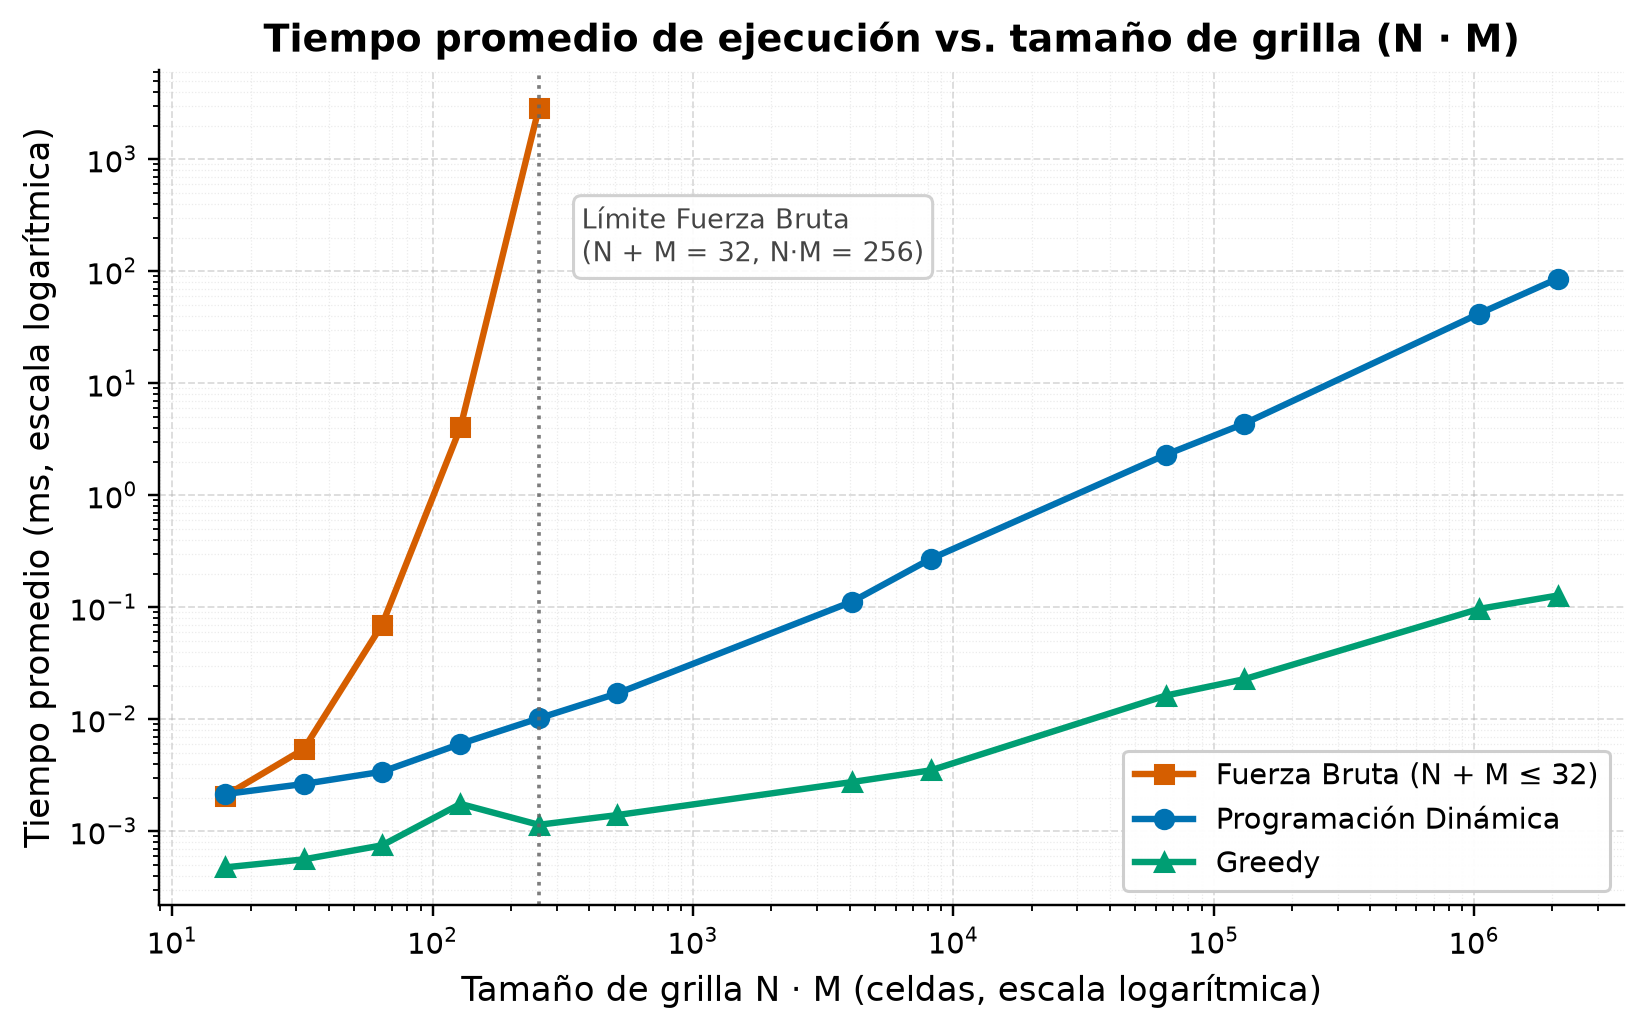
\includegraphics[width=0.8\textwidth]{../code/grid_pathfinding/data/plots/tiempo_vs_nm.png}
\caption{Tiempo promedio vs $N\cdot M$ (escala log en $y$).}
\label{fig:tiempo}
\end{figure}

\paragraph{Memoria.} En la Figura~\ref{fig:mem} la fuerza bruta y greedy muestran incremento 0 KB en todas las corridas, ya que usan memoria $O(N+M)$ que no supera la paginación. DP usa una tabla de $N\cdot M$ y su incremento promedio crece: 128 KB con $N=64$, 2676 KB con $N=256$ y 41520 KB con $N=1024$ (máximo 55356 KB). Para $N\le16$ el valor es 0, por lo que solo es representativo en grillas grandes.

\begin{figure}[h]
\centering
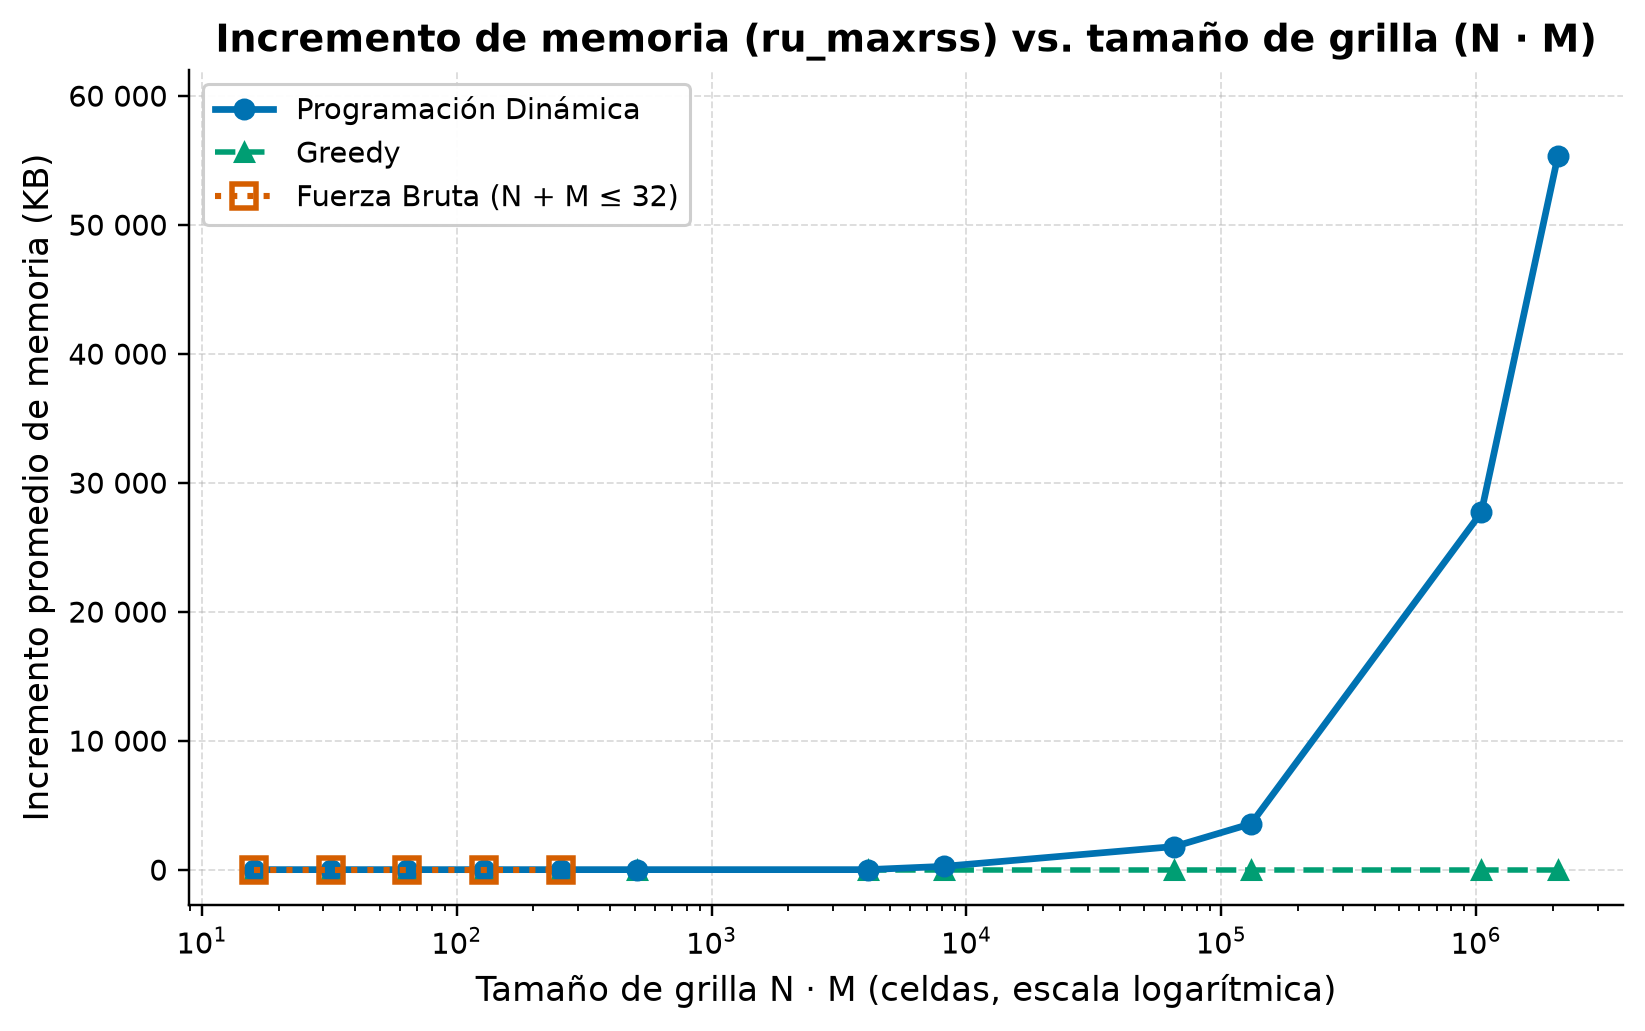
\includegraphics[width=0.8\textwidth]{../code/grid_pathfinding/data/plots/memoria_vs_nm.png}
\caption{Incremento de memoria (\texttt{mem\_kb}) vs $N\cdot M$.}
\label{fig:mem}
\end{figure}

\paragraph{Calidad de Greedy.} Greedy encontró solución en el 86,8\% de las instancias (250 de 288), mientras DP y fuerza bruta la encontraron en todas. Fuerza bruta coincidió con DP en el puntaje en las 120 instancias donde corrió. La brecha $\Delta=\text{Score}_{DP}-\text{Score}_{Greedy}$ (Figura~\ref{fig:brecha}, solo instancias donde greedy halla solución) nunca fue negativa, mínimo 0, mediana 1481,5 y promedio 61786. Crece con el tamaño y con el dominio: en D10 va de 5,6 ($N=4$) a 5277 ($N=1024$), y en D1000 de 354,7 a 523118. Es decir, el error absoluto escala con el rango de valores y con la cantidad de celdas.

\begin{figure}[h]
\centering
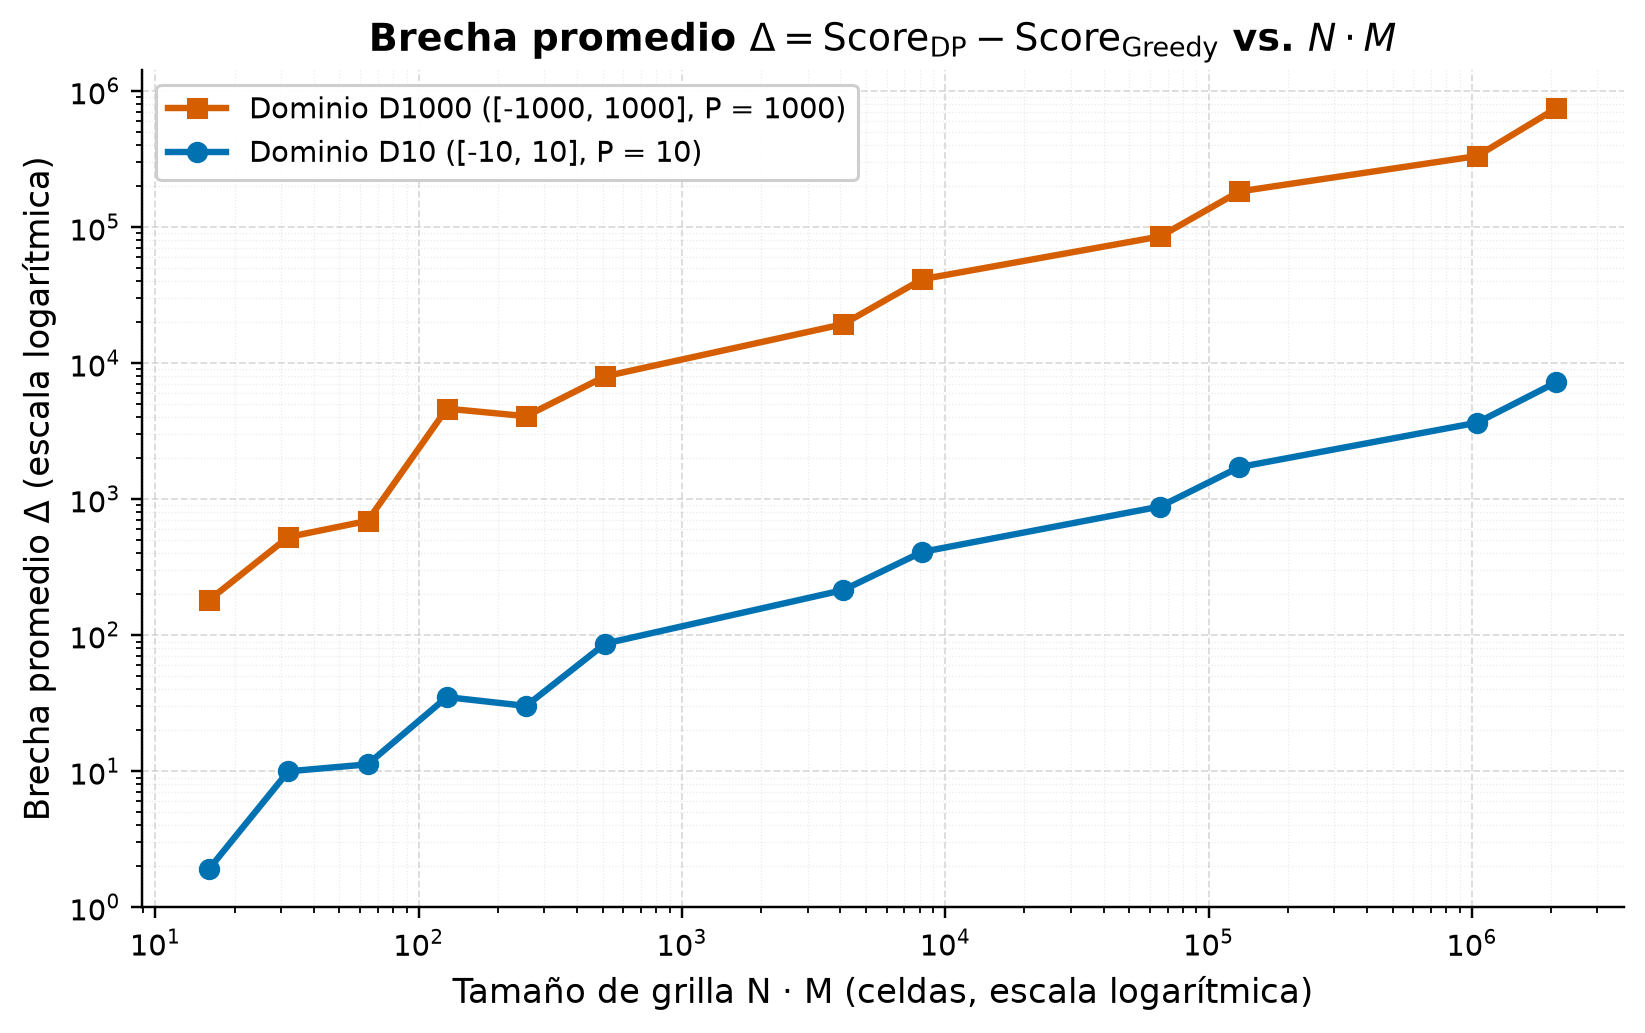
\includegraphics[width=0.8\textwidth]{../code/grid_pathfinding/data/plots/brecha_delta_vs_nm.png}
\caption{Brecha $\Delta$ vs $N\cdot M$ para D10 y D1000.}
\label{fig:brecha}
\end{figure}

\paragraph{Fallas de Greedy.} La Figura~\ref{fig:falla} muestra la tasa de falla por tipo de grilla. En \textit{libre} es 0\% en ambos dominios y en \textit{minas} 0\% (D10) y 2,8\% (D1000). Fallan mucho más las grillas con muros: \textit{murallas} 22,2\% (D10) y 33,3\% (D1000), y \textit{mixta} 33,3\% (D10) y 13,9\% (D1000). Esto es esperable: greedy no retrocede, por lo que un muro o mina letal puede dejarlo atrapado aunque exista camino. Por tamaño, la falla no muestra tendencia clara (12,5\% con $N=4$, 20,8\% con $N=64$, 6,3\% con $N=256$, 12,5\% con $N=1024$), así que el tipo de grilla pesa más que el tamaño; el dominio afecta distinto según el tipo con 36 instancias por celda, por lo que las diferencias entre D10 y D1000 deben leerse con cautela.

\begin{figure}[h]
\centering
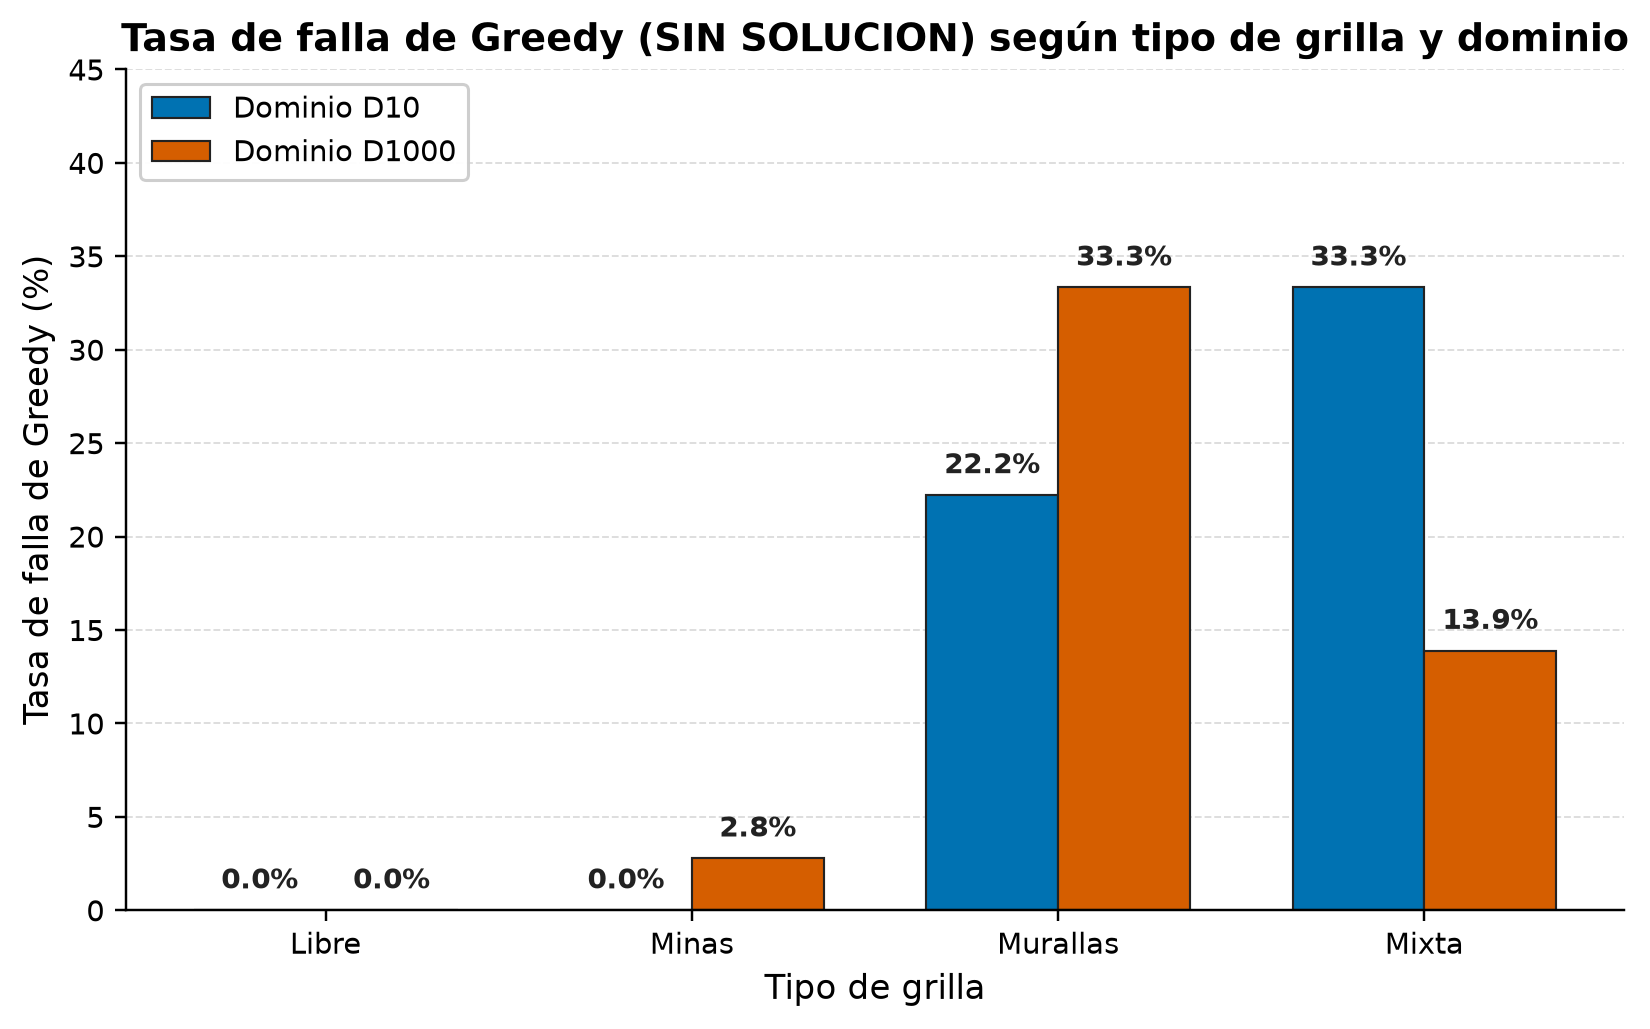
\includegraphics[width=0.8\textwidth]{../code/grid_pathfinding/data/plots/tasa_falla_greedy.png}
\caption{Tasa de falla de Greedy por tipo de grilla y dominio.}
\label{fig:falla}
\end{figure}
